% https://github.com/martinhelso/MathDept


\documentclass[UKenglish]{beamer}


\usetheme[NoLogo]{MathDept}


\usepackage[utf8]{inputenx} % For æ, ø, å
\usepackage{babel}          % Automatic translations
\usepackage{csquotes}       % Quotation marks
\usepackage{microtype}      % Improved typography
\usepackage{amssymb}        % Mathematical symbols
\usepackage{mathtools}      % Mathematical symbols
\usepackage[absolute, overlay]{textpos} % Arbitrary placement
\setlength{\TPHorizModule}{\paperwidth} % Textpos units
\setlength{\TPVertModule}{\paperheight} % Textpos units
\usepackage{tikz}
\usetikzlibrary{overlay-beamer-styles}  % Overlay effects for TikZ


\author{William Hirst}
\title[Supervised Learning in HEP]{Application of Supervised Machine Learning to the Search for New Physics in ATLAS data}
\subtitle{A Study of Ordinary Dense, Parameterized and Ensemble Networks and their Application to High Energy Physics}


\begin{document}


\section{Overview}

\begin{frame}{Outline}
    \tableofcontents
\end{frame}

\SubSectionPage{Overview}

\section{Introduction $\&$ Motivation}
\begin{frame}{Outline}
    \tableofcontents[currentsection]
\end{frame}

\subsection{Why apply machine learning to HEP problems?}
\begin{frame}{Why apply machine learning to HEP problems?}
 
\end{frame}


\subsection{How do we search for new physics?}
\begin{frame}{How do we search for new physics?}
 
\end{frame}

\section{The Implementation}
\begin{frame}{Outline}
    \tableofcontents[currentsection]
\end{frame}

\subsection{A summary of the applied methods}
\begin{frame}{A summary of the applied methods}
    \emph{Three} neural network variants
    \begin{itemize}
        \item Ordinary dense neural network
        \item Ensemble networks utilizing Local-Winner-Takes-All (LWTA) layers
        \item Parameterized neural networks (PNN)
    \end{itemize}
    \emph{One} boosted decision tree method
    \begin{itemize}
        \item XGBoost using default settings
    \end{itemize}
\end{frame}

\subsection{How are the methods compared?}
\begin{frame}{How are the methods compared?}

\end{frame}

\subsection{Training strategy}
\begin{frame}{Training strategy}
 
\end{frame}


\section{Methods $\&$ Results}
\begin{frame}{Outline}
    \tableofcontents[currentsection]
\end{frame}

\subsection*{An introduction and study of each method}
\SubSectionPage{An introduction and study of each method}


\begin{frame}{Ordinary dense neural network}
    
\end{frame}


\begin{frame}{Ensemble methods - LWTA}
    \begin{itemize}
        \item Dropout
        \item What is LWTA?
        \item Competing nodes - Units
        \item Pattern specific pathways
    \end{itemize}    
    \begin{textblock}{0.58}(0.2, 0.365)
        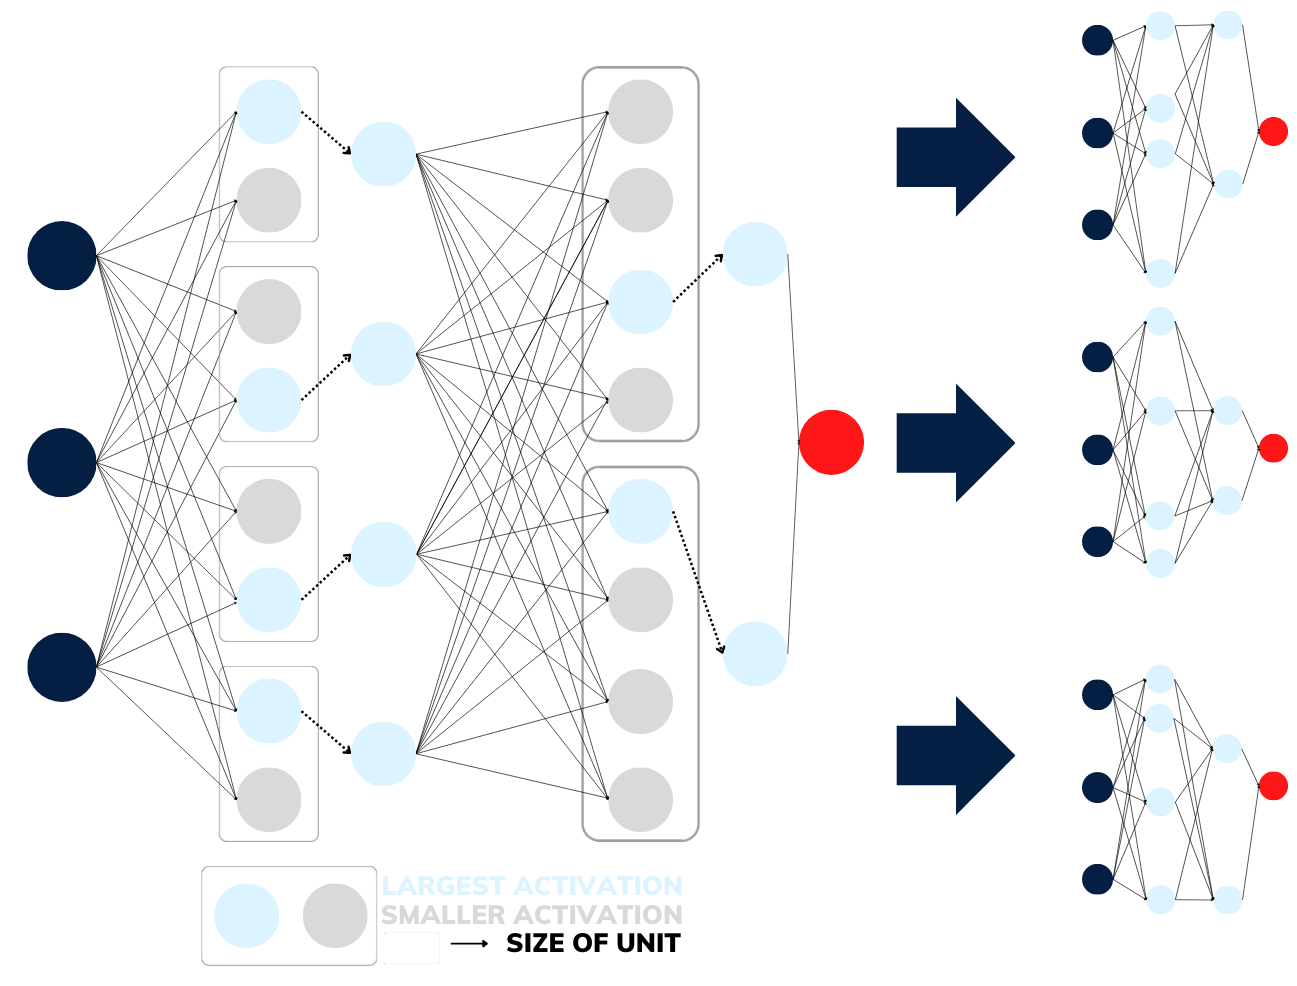
\includegraphics[width = \textwidth]{figures/Max_out}
    \end{textblock}
\end{frame}

\begin{frame}{Channel-Out, SCO and Maxout}
    \center
        \begin{table}
            $
            \begin{array}{cccc}
                \hline \text { Layer } & \text { Separate Weights $\&$ Biases } & \text { Static Units }\\
                \hline\hline\text{Channel-Out} & \text{Yes} &  \text{Yes}  \\
                \text { SCO } &  \text{Yes} &  \text{No}  \\
                \text{ Maxout } &  \text{No} &  \text{Yes}   \\
                \hline
            \end{array}
            $
        \end{table}
    \begin{textblock}{0.8}(0.1, 0.45)
        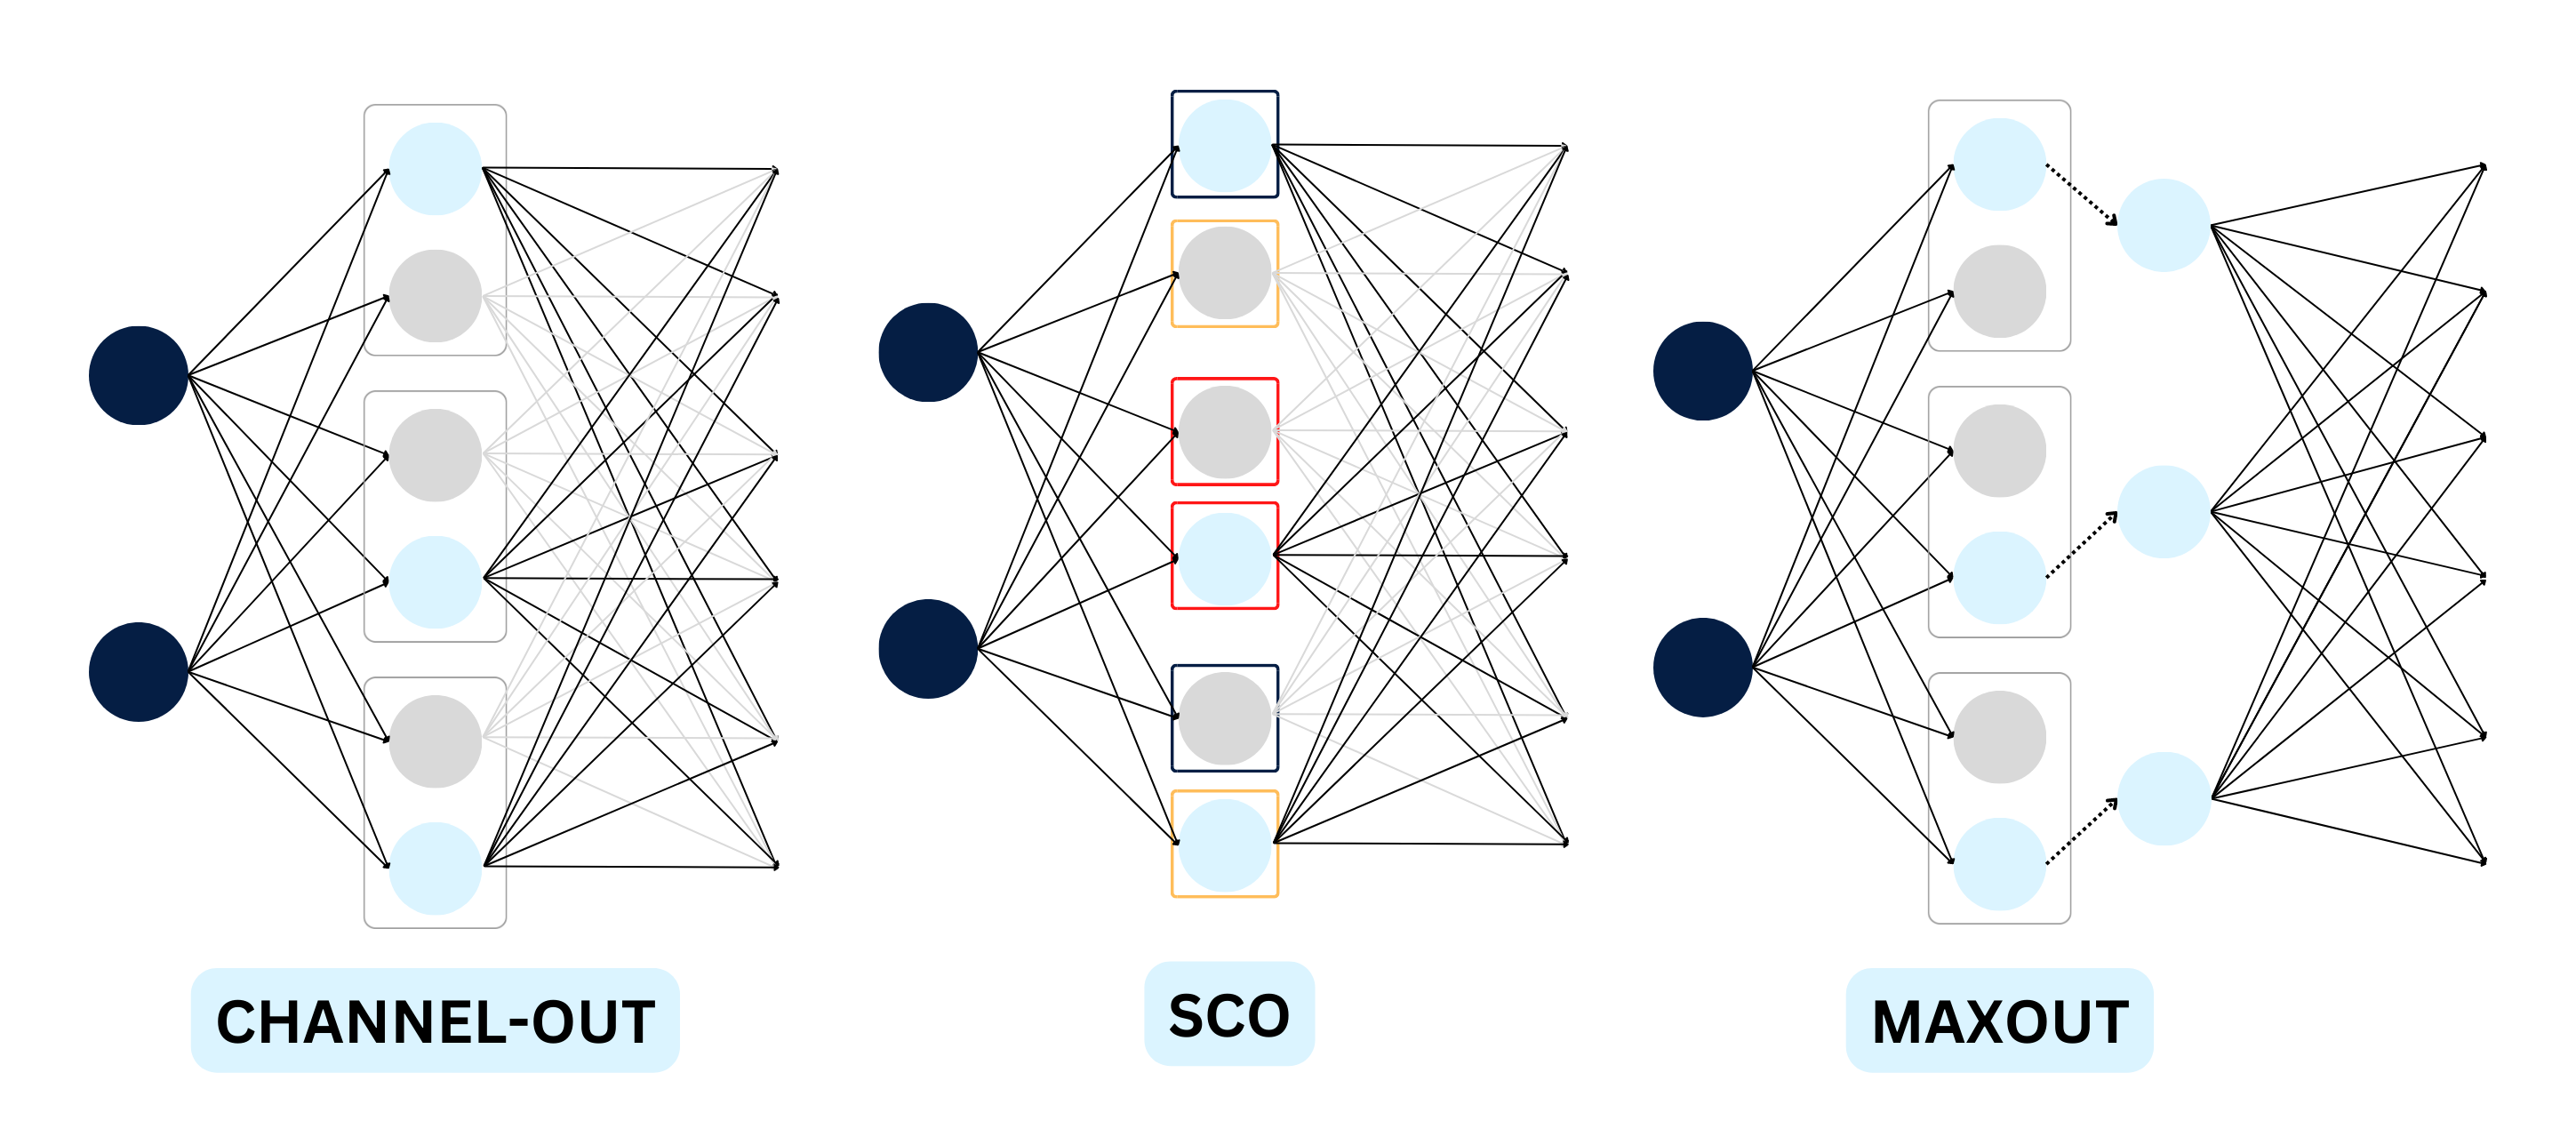
\includegraphics[width = \textwidth]{figures/EnsembleComp}
    \end{textblock}
\end{frame}


\begin{frame}{Parameterized neural network}
    
\end{frame}


\begin{frame}{Boosted decision trees - XGBoost}
 
\end{frame}
\subsection{Comparing the methods}

\subsection{Compare the methods to previous analysis}

\section{Conclusion $\&$ Outlook}
\begin{frame}{Outline}
    \tableofcontents[currentsection]
\end{frame}




\section{References}


\begin{frame}[allowframebreaks]{References}
    \begin{thebibliography}{}

        % Article is the default.
        \setbeamertemplate{bibliography item}[book]

        \bibitem{Hartshorne1977}
        Hartshorne, R.
        \newblock \emph{Algebraic Geometry}.
        \newblock Springer-Verlag, 1977.

        \setbeamertemplate{bibliography item}[article]

        \bibitem{Helso2020}
        Helsø, M.
        \newblock \enquote{Rational quartic symmetroids}.
        \newblock \emph{Adv. Geom.}, 20(1):71--89, 2020.

        \setbeamertemplate{bibliography item}[online]

        \bibitem{HR2018}
        Helsø, M.\ and Ranestad, K.
        \newblock \emph{Rational quartic spectrahedra}, 2018.
        \newblock \url{https://arxiv.org/abs/1810.11235}

        \setbeamertemplate{bibliography item}[triangle]

        \bibitem{AM1969}
        Atiyah, M.\ and Macdonald, I.
        \newblock \emph{Introduction to commutative algebra}.
        \newblock Addison-Wesley Publishing Co., Reading, Mass.-London-Don
        Mills, Ont., 1969

        \setbeamertemplate{bibliography item}[text]

        \bibitem{Artin1966}
        Artin, M.
        \newblock \enquote{On isolated rational singularities of surfaces}.
        \newblock \emph{Amer. J. Math.}, 80(1):129--136, 1966.

    \end{thebibliography}
\end{frame}


\end{document}